% !TeX root = ../main.tex
% Add the above to each chapter to make compiling the PDF easier in some editors.

\chapter{The RTG \textit{Tachyon} Engine} \label{Tachyon}

Rendering optimizations can only be implemented if there actually is a renderer at hand. In order to see how the chosen approaches would perform in an engine intended for productive use and industrial applications, rather than an ad hoc renderer only built for some specific tests, \textit{Tachyon} was chosen, an engine currently in development at RTG Echtzeitgraphik GmbH. \textit{Tachyon} uses a fully Vulkan based forward renderer (internally called rtvklib) with support for multiple viewports of various types, including an OpenVR based virtual reality path, an optional physically-based shader pipeline, a user interface module, a network module and a physics module with more extensions on the development schedule for the future. The renderer integrates Vulkan version 1.1.85 and up and OpenVR version 1.4.18 and up with support for all major SteamVR headsets at the time of writing, including roomscale tracking of the Valve Index, HTC Vive and Vive Pro, the Windows Mixed Reality series and Oculus Rift series. 

\section{Render setup} 
As typical for the verbose nature of Vulkan, render initialization starts with the creation of all necessary basic Vulkan resources such as descriptors, descriptor sets, activation of a minimal set of Vulkan extensions and layers and device enumeration. 
More specific to \codeword{rtvklib}, multiple Vulkan pipelines are active by default:
\begin{itemize}
\item a material pipeline offering support for a Phong and a PBR shader as well as geometry and index buffers of arbitrary size
\item a skybox pipeline with a simplified skybox shader
\item a point cloud pipeline, primarily to allow rendering of LiDAR scan data
\end{itemize}
To facilitate rendering into multiple viewports, \textit{Tachyon} uses the concept of render targets. Each render target can reference an arbitrary subset of pipelines, comes with its own set of Vulkan framebuffers, command buffers and render pass and its own virtual camera. 
Whenever any 3D object is to be loaded, \codeword{rtvklib} uses several manager classes to keep track of the various resource types needed for an object. There are managers for geometry, materials, textures and instances among other types. When an object is loaded, the former three hold the respective buffers. When an object is to be rendered, it first needs to be instanced, handled by the latter. An instance references the various geometry and materials of the original object again, but also holds data specific to individual objects in the virtual world, such as transforms or bounding geometry. 

The renderer initialization also encompasses virtual reality through OpenVR. Given a valid OpenVR environment and HMD is detected, a special render target is created with a Vulkan renderpass for multiple views and the respective resources. Resources include a framebuffer with one layer for each eye, created with the rendering resolution returned by OpenVR after querying \codeword{IVRSystem::GetRecommendedRenderTargetSize()} and using 4x multisampling as is often recommended for virtual reality applications to minimize aliasing without obscene cost (see for example \cite{Vlachos.2015} p. 25f, \cite{Porter.2017}, \cite{Carmack.2016}, \cite{VisCircleGmbH.2018}, \cite{Pettit.2017}). 

All run-time relevant vector and matrix math in the renderer and the presented optimization implementations use the free MPL2 licenses Eigen 3.3 math library. Eigen was chosen for its extensive feature set and its special focus on high performance using SIMD vectorization including all current forms of SSE and AVX among others\cite{Guennebaud.2010}.

\section{Render loop} 
After all startup and initialization is done, the engine's render loop executes \codeword{VKRenderer}'s \codeword{Update()} and \codeword{RenderFrame()} functions back to back. The flows of these are shown in \autoref{fig:lst_VKRenderer_Update} and \autoref{fig:lst_VKRenderer_RenderFrame}, respectively. 

\begin{figure}[htb]
  \centering
  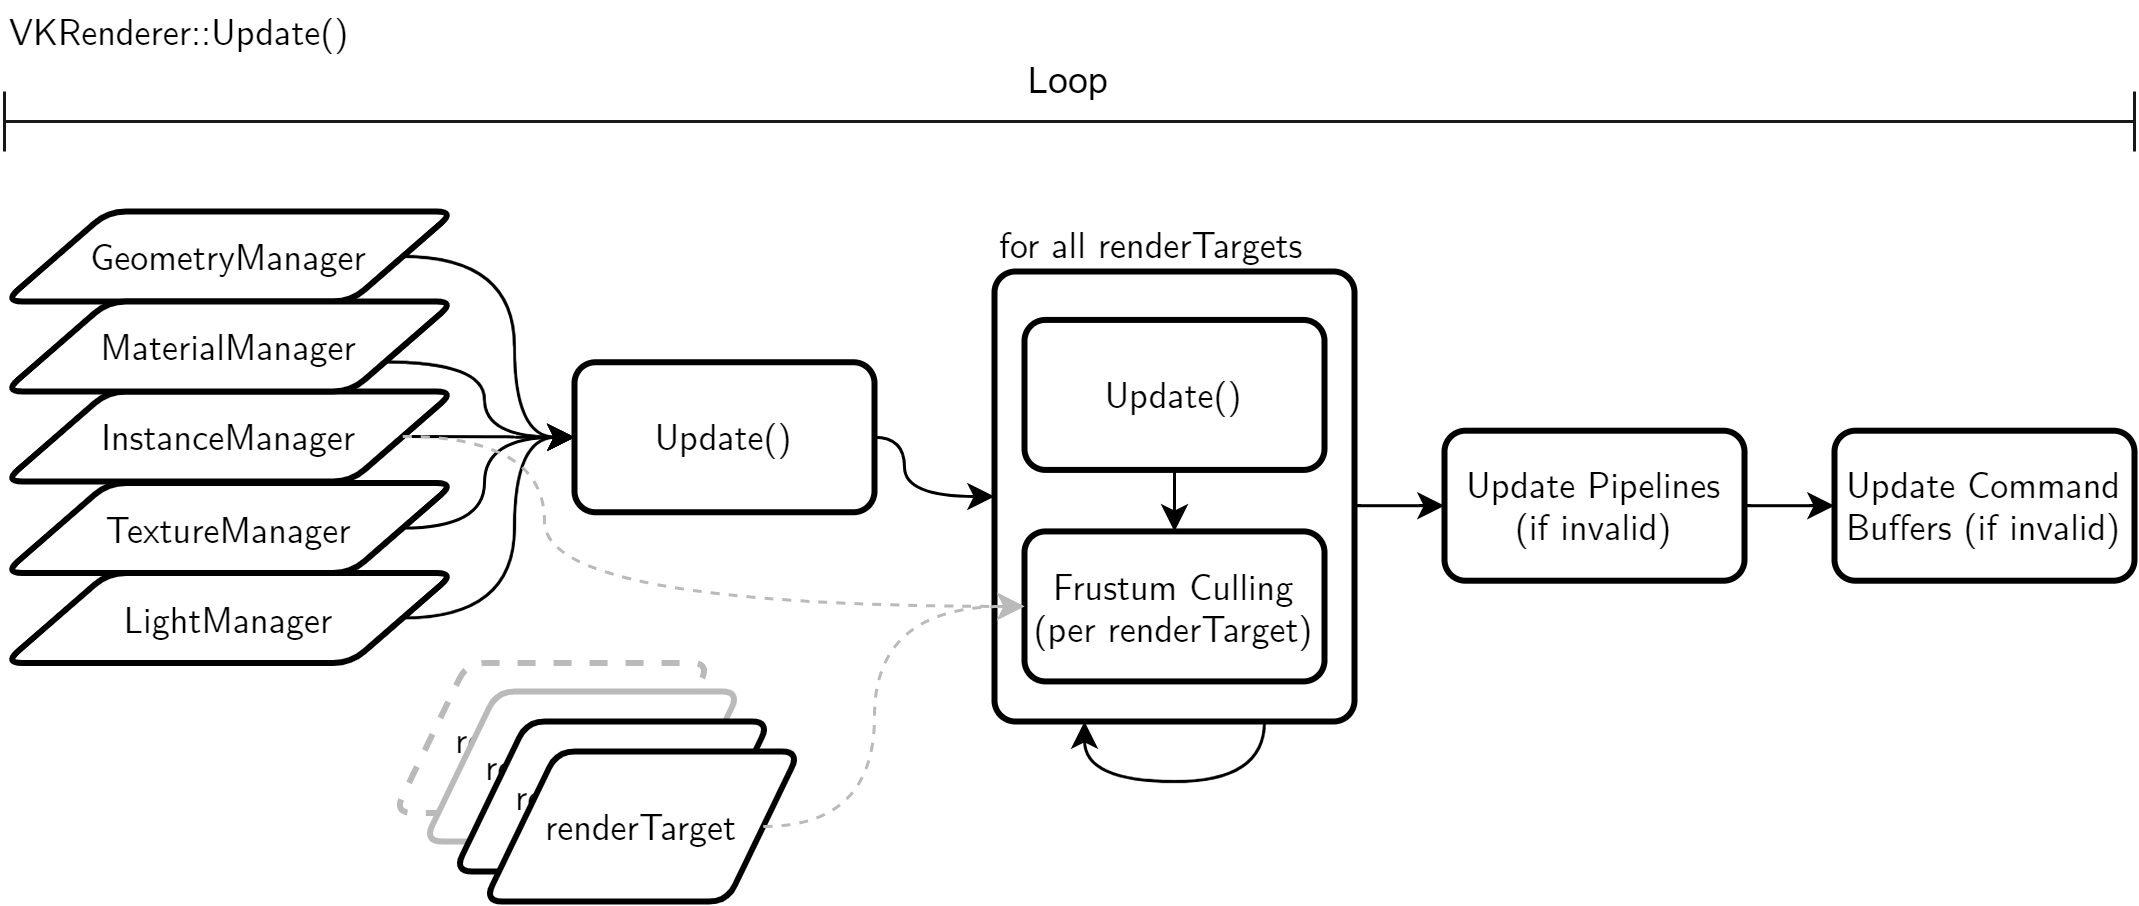
\includegraphics[width=0.9\textwidth]{pictures/Tachyon_VKRenderer_Update}
  \caption[VKRenderer's Update]{Renderer update function \textcolor{red}{[TODO: autoref code snippet in appendix]}}\label{fig:lst_VKRenderer_Update}
\end{figure} 

\iffalse
\begin{figure}[htb]
  \centering
  \begin{tabular}{c}
  \begin{lstlisting}[language=C++]
void VKRenderer::Update()
{
	mRenderMutex.lock();
	mGeometryManager->Update();
	mMaterialManager->Update();
	mInstanceManager->Update();
	mTextureManager->Update();
	mLightManager->Update();
	mPointCloud->Update();
	UpdateGlobalParamsBuffer();

	for (auto renderTarget : mRenderTargets)
	{
		renderTarget->Update();
		mInstanceManager->FrustumCulling(renderTarget); 
	}

	if (mPipelinesInvalid) UpdateRenderPipelines();
	if (mCommandBuffersInvalid) UpdateCommandBuffers();
	mRenderMutex.unlock();
}
  \end{lstlisting}
  \end{tabular}
  \caption[VKRenderer's Update]{Renderer update function \textcolor{red}{[TODO: move to appendix, replace with compact flowchart?]}}\label{fig:lst_VKRenderer_Update}
\end{figure}
\fi

\codeword{VKRenderer::Update()} first prompts all aforementioned managers to update their databases, buffers and anything else they hold in case they are dirty. Then it prompts each render target to update, which may involve camera transformation updates and buffer synchronization for example. Also for each render target, the loop will then have the instance manager perform a frustum culling pass, which will for this target save a conservative list of draw call information for objects visible by this target's camera viewpoints. 
If any of these updates and culling passes set a pipeline or command buffer state invalid, these will be rebuilt accordingly.  

\begin{figure}[htb]
  \centering
  \begin{tabular}{c}
  \begin{lstlisting}[language=C++]
void VKRenderer::RenderFrame()
{
	if (!mDevice)
		return;

	mRenderMutex.lock();
	for (auto renderTarget : mRenderTargets)
	{
		renderTarget->RenderFrame();
	}
	mRenderMutex.unlock();
}
	\end{lstlisting}
  \end{tabular}
  \caption[VKRenderer's RenderFrame]{Renderer frame render function\textcolor{red}{[TODO: move to appendix, replace with compact flowchart?]}}\label{fig:lst_VKRenderer_RenderFrame}
\end{figure}

\codeword{VKRenderer::RenderFrame()} simply prompts each render target to perform its per-frame rendering operations, be it regular monoscopic output for a traditional viewport or pose tracking and stereoscopic composition for a virtual reality target. 

\subsection{VR render loop}
The virtual reality render target's \codeword{RenderFrame()} function is rather straight-forward. 
As long as the target and compositor are active, it updates the OpenVR device poses and virtual camera transforms. It then renders the stereoscopic views, resolves the multisampling layers into single sample and finally submits both eyes' images to SteamVR, which serves as the chosen OpenVR compatible compositor on Windows systems. \\

As the VR view essentially moves constantly, its render target needs to update its Vulkan \codeword{VkCommandBuffer} every frame. This is done by setting the \codeword{mCommandBuffersInvalid} flag which has the renderer call \codeword{UpdateCommandBuffers()} which in turn prompts each render target to \codeword{RecordCommandBuffers()}. For each of the VR render target's command buffers this is a simple loop through the \codeword{RecordDrawCommand()}s of the pipelines assigned to this render target between the Begin and End commands of the command buffer and render pass. The draw command recording function has the respective pipeline query the \codeword{InstanceManager} for its post-culling draw command set and writes the contained entries as \codeword{vkCmdDrawIndexedIndirect()} draw calls. 

\begin{figure}[htb]
  \centering
  \begin{tabular}{c}
  \begin{lstlisting}[language=C++]
void OpenVR::RecordCommandBuffers(uint32_t passId)
{
	for (uint32_t i = 0; i < mCommandBuffers.size(); ++i)
	{
		VkCommandBufferBeginInfo beginInfo = {};
		[...]
		vkBeginCommandBuffer(mCommandBuffers[i], &beginInfo);

		VkRenderPassBeginInfo renderPassInfo = {};
		[...]
		vkCmdBeginRenderPass(mCommandBuffers[i], &renderPassInfo, 
		VK_SUBPASS_CONTENTS_INLINE);

		for (auto renderPipeline : mRenderPipelines)
		{
			renderPipeline->RecordDrawCommand(mCommandBuffers[i], 
			passId);
		}

		vkCmdEndRenderPass(mCommandBuffers[i]);
	}
}
	\end{lstlisting}
  \end{tabular}
  \caption[OpenVR render target's RecordCommandBuffers]{OpenVR command buffer recording function \textcolor{red}{[TODO: move to appendix, replace with compact flowchart?]}}\label{fig:lst_OpenVR_RecordCommandBuffers}
\end{figure}

What's more, as seen in \autoref{fig:lst_OpenVR_RenderFrame}, \textcolor{red}{[TODO: briefly describe OpenVR::RenderFrame]}. \\

\begin{figure}[htb]
  \centering
  \begin{tabular}{c}
  \begin{lstlisting}[language=C++]
void OpenVR::RenderFrame()
{
	if (!mIsActive || !vr::VRCompositor())
	{
		return;
	}

	// update ovr poses and camera transforms
	UpdateHMDMatrixPose();
	UpdateCameras();

	// render stereo
	[...]
	submitInfo.pCommandBuffers = &mCommandBuffers[mCurrentFrame];
	vkQueueSubmit(queue, 1, &submitInfo, mInFlightFences[mCurrentFrame]);

	// blit/resolve array layers
	[...]
	submitInfo.pCommandBuffers = &mResolveCommandBuffer;
	vkQueueSubmit(queue, 1, &submitInfo, VK_NULL_HANDLE);

	// Submit to SteamVR
	[...]
	for (int i = 0; i < 2; i++)
	{
		vulkanData.m_nImage = (uint64_t)mResolveImage[i];
		vr::VRCompositor()->Submit(static_cast<vr::EVREye>(i), 
		&texture, &bounds);
	}
}
	\end{lstlisting}
  \end{tabular}
  \caption[OpenVR render target's RenderFrame]{OpenVR frame render function \textcolor{red}{[TODO: move to appendix, replace with compact flowchart?]}}\label{fig:lst_OpenVR_RenderFrame}
\end{figure}

\textcolor{red}{[TODO: overview illustration aka flowchart?]}